\chapter{Entity master data} \label{ch:entitymasterdata}


% General motivation
Under current European reporting regimes such as EMIR or SFTR the identification of individual counterparties is based on the Legal Entity Identifier (LEI). The LEI is a string of twenty seemingly random alphanumeric values with no immediately recognisable meaning unless it is augmented with further reference data. This includes, among others, the name, country or sector of an entity. Although  some reference data such as sector and country of a counterparty is also reported under EMIR and SFTR, there are several analytical use cases, which benefit from a well-curated entity master data set. This pertains mostly to the calculation of group-specific market indicators such as aggregates based on countries, sectors or business models, which is a necessary data processing step for the generation of dashboards and market reports. To facilitate such analyses, the \emph{fincommons} Python package includes functions for the creation of such an entity master data set.

\begin{figure}[h]
	\centering
	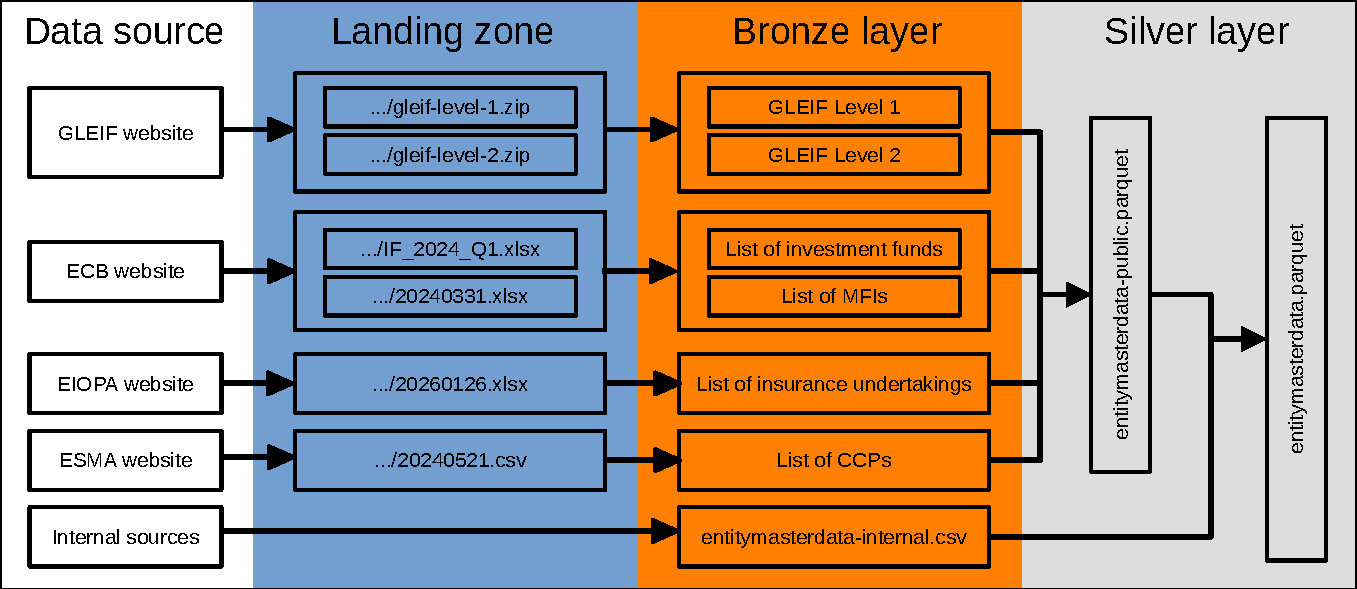
\includegraphics[height=6cm]{entity-master-data-architecture}
	\caption{Data pipeline of entity master data.\label{fig:function_entitymasterdata}}
\end{figure}

% General implementation
Within the \emph{fincommons} framework, the creation of an entity master data set follows \textcite{ESMA.2018} and \textcite{Lenoci.2021}.\footnote{More recently, also see \textcite{Pezzini.2024}.} The corresponding data pipeline is shown in figure \ref{fig:function_entitymasterdata} and consists of the following steps:
%
\begin{itemize}
	\item Load data from various public sources (ECB, EIOPA, ESMA, GLEIF) into the respective folders of the landing zone. GLEIF describes who an entity is and how it is related to other entities, and the sectoral registers state what it does: the ECB lists of investment funds and of monetary financial institutions, the EIOPA registers of insurance undertakings and of institutions for occupational retirement provision (IORPs), and the ESMA list of central counterparties. Between them they fill the field SECTOR, whose values are listed in table \ref{tab:entitymasterdata-sector}.\footnote{The target folders are listed in the module's README file.} Two of these are downloaded by the package. The GLEIF golden copies are fetched from a link that has to be given to the download, because GLEIF publishes no stable address for the most recent release and changes it with every one of them. The list of central counterparties is taken from a public GitHub repository that keeps the information in machine-readable form, since ESMA publishes its registers of authorised and of recognised counterparties as pdf files, which cannot reasonably be read. The ECB and EIOPA registers cannot be reached through a standardised interface at all and have to be placed in the landing zone by hand, under the names the module's README file states, from which the reference date of the register is read.

A download leaves the register or nothing. The answer is written under a temporary name and put in place only once it is complete, so an interrupted download leaves nothing behind under the name the Bronze import reads. An error answer, and an answer that is served with a success status but does not open as the archive it should be, are refused for the same reason: a GLEIF link that has gone stale answers with an error page, which would otherwise be stored under the name of the register and imported as if it were one.
	\item The registers are imported into the Bronze layer to make them queryable. This entails that the data is converted to Parquet from the formats the publishers use: the GLEIF golden copies are read from the zipped CSV files that GLEIF publishes alongside its XML ones, the ECB and EIOPA registers from the Excel workbooks they are handed out as, and the list of CCPs from a CSV file. No major changes to the schema are made so that all potentially useful information remains available.
	\item Optional: Prepare internal entity master data so that it conforms to the structure described in the annex document \emph{Annex - Entity Master Data - Data Dictionary.xlsx}. This data could be obtained from supervisory or proprietary sources as in, e.g., \textcite{Lenoci.2021}. Save the result as a CSV-file in the Bronze layer as specified in the directory tree in figure \ref{fig:dirstruct_entitymasterdata}. The CSV file format was chosen, because it allows to impose a schema, which supports data validation and contributes to greater stability of the data pipeline. The file is checked before it is combined with anything: a file without the field LEI, one with a field the entity master data set does not have, and one that describes the same LEI twice are refused, because the first would displace nothing, the second would lose what it says under the unknown field when the table is written, and the third would leave the choice between the two descriptions to the order in which Spark happens to read them. An LEI that does not have the form of one is kept and named in a warning.
	\item In case internal data is used, the public and internal data sets are combined and de-duplicated. The current implementation of \emph{fincommons} prefers internal data over public data. Thus, data engineers should ensure that when internal data is used, it is \emph{at least} of the same quality than the public data. This is because the processing function only keeps the internal information when there are duplicated values in the merged data set.\footnote{One approach to achieve this is to build on the public data set and enrich it with internal information before saving in the Bronze layer from where it is combined with the public data again. Although this leads to computational redundancies, it ensures that the \emph{fincommons} code base can be used within any organisation to produce the best internationally harmonised entity master data set}.
	\item Add two catch-all entities, which serve at later stages of a data processing pipeline. The entity ``Other'' collects what an aggregation does not show on its own -- the reporting counterparties below the top fifteen of the data quality monitoring of EMIR and SFTR are filed under it, for example, and a chart whose legend names the top five categories puts the rest there -- and the entity ``Unknown'' takes what could not be identified at all, which makes data quality issues easy to spot. The package adds both to the entity master data set itself, under the LEIs \verb|XOTHERX0000000000064| and \verb|XUNKNOWNX00000000025|. Both have the form ISO 17442 prescribes, so that they pass every check an LEI is put to: eighteen characters, padded with zeros, followed by two check digits that make the whole number leave a remainder of one on division by 97. The first four characters of an LEI name the Local Operating Unit that issued it, and none has issued one under \verb|XOTH| or \verb|XUNK|: of the 3,424,918 LEIs of the GLEIF golden copy of 8 September 2026, 521 begin with an X and none with either prefix. A proprietary list that describes one of the two, with a sector of its own for instance, takes precedence over the package's description as it does for any other entity.
\end{itemize}


% Sector codes
\begin{table}[h]
	\centering
	\begin{tabular}{l l l p{6.2cm}}
		\hline
		SECTOR & Rank & Register & Content \\
		\hline
		\verb|CCP|  & 1 & ESMA   & \raggedright Central counterparty. The field SUBSECTOR distinguishes an authorised EU counterparty (\verb|EUCCP|) from a recognised third country one (\verb|T1CCP|, \verb|T2CCP|). \tabularnewline
		\verb|INUN| & 2 & EIOPA  & Insurance undertaking. \\
		\verb|ORPI| & 3 & EIOPA  & Institution for occupational retirement provision. \\
		\verb|CB|   & 4 & ECB    & Central bank. \\
		\verb|CDTI| & 4 & ECB    & Credit institution. \\
		\verb|OFI|  & 4 & ECB    & Other institution on the list of monetary financial institutions. \\
		\verb|MMF|  & 4 & ECB    & Money market fund. \\
		\verb|UCIT| & 5 & ECB    & Investment fund compliant with the UCITS directive. \\
		\verb|AIFD| & 5 & ECB    & Alternative investment fund. \\
		\verb|INVF| & 5 & ECB    & Investment fund the register reports neither of the two about. \\
		\hline
	\end{tabular}
	\caption{Values of the field SECTOR, with the register each is taken from and the rank that settles which one is kept where an entity stands in more than one of them.\label{tab:entitymasterdata-sector}}
\end{table}

An entity can appear in several of these registers, and the rank in table \ref{tab:entitymasterdata-sector} decides which description is kept. The ordering is by how much the register says: a central counterparty is licensed as a credit institution in a number of member states and would otherwise carry that description, and a money market fund stands on the list of investment funds as well. Two of the ranks deserve a word. The insurance register is placed above the register of institutions for occupational retirement provision because a number of entities stand in both -- the Pensionskassen constituted as insurers among them -- and the insurance register states the authorisation the entity holds, whereas the IORP register states an activity carried on under it. The four values the list of monetary financial institutions supplies share one rank, and so do the three the list of investment funds supplies, since each set comes from one register and is mutually exclusive within it. A register can also carry the same LEI twice -- a central counterparty authorised under more than one heading stands in the list of CCPs once per heading, and an institution licensed in several member states stands in the list of MFIs once per state -- and the rank settles nothing there. The choice therefore runs on through the sector and the subsector, preferring a row that states one to a row that does not and otherwise taking the alphabetical one. That decides nothing anyone asked about, but it decides it the same way on every run, which is what the table has to do to be comparable with itself. The three fund codes are read off what the register says about compliance with the UCITS directive; the field IF\_UCITS\_COMPL keeps that statement itself, which is not the same thing as the sector, and SUBSECTOR carries the investment policy the fund pursues.

All of this rests on the LEI being written the same way in every register, since the registers are joined on it as text and an LEI written differently is a different key: it matches no entity of the GLEIF data, and the entity it stands for goes without the sector the register would have given it. The registers do not always write it the same way. The ECB and EIOPA registers are converted from spreadsheets by hand and the list of central counterparties is compiled from ESMA's pdf files, and in September 2026 the list of central counterparties carried six LEIs with a trailing space and the IORP register three in lower case. Joined as they stand, they leave two central counterparties, KDPW\_CCP and Euronext Clearing Athens, and three Italian pension funds without a sector, and with them their positions in every sector aggregate of the EMIR and SFTR data. Every LEI is therefore written the way GLEIF writes it before it is joined -- blanks, including the non-breaking space a spreadsheet leaves, removed and letters put in upper case -- in the registers, in the GLEIF data itself and in a proprietary list alike. Since an LEI contains neither blanks nor lower-case letters, this changes no LEI that was well-formed. One that still does not have the form ISO 17442 gives it, eighteen letters or digits followed by two check digits, is kept but named in a warning together with the register it came from.

Figure \ref{fig:dirstruct_entitymasterdata} shows the directory structure that is used for the implementation of this pipeline. The Silver layer holds two tables addressed by path, \emph{public} for the data set built from the public registers alone and \emph{main} for the one a proprietary list has been put in front of.

Either table can be written as Parquet or as Delta, and the update functions take the choice as an argument. Parquet is the default, because it is the format every engine reads without a further dependency, which is what a table meant to be shared should be. Delta buys two things Parquet does not have and is worth choosing where they matter: a rebuild replaces the table in a single transaction, so that a reader either sees the previous version in full or the new one and never the half-written state that overwriting a set of Parquet files in place would leave behind, and the previous versions of the table remain readable. The table is read back in whichever format it was written in, so the choice does not have to be repeated when it is queried. Switching an existing table from Parquet to Delta is the one direction that needs a hand, since Delta will not adopt Parquet files it has no transaction log for: the directory has to be deleted before the first Delta update.

% Directory tree
\begin{figure}[h!]
	\centering
	\begin{subfigure}[t]{0.32\textwidth}
		\centering
		\begin{forest}
			for tree={
				%font=\ttfamily,
				grow'=0,
				child anchor=west,
				parent anchor=south,
				anchor=west,
				calign=first,
				edge path={
					\noexpand\path [draw, \forestoption{edge}]
					(!u.south west) +(7.5pt,0) |- node[fill,inner sep=1.25pt] {} (.child anchor)\forestoption{edge label};
				},
				before typesetting nodes={
					if n=1
					{insert before={[,phantom]}}
					{}
				},
				fit=band,
				before computing xy={l=15pt},
			}
			[landing
			[ecb
			[investment\_fund
			[IF\_2025\_Q3.xlsx]
			]
			[mfi
			[20250130.xlsx]
			]
			]
			[eiopa
			[insurance\_undertaking
			[20250202.xlsx]
			]
			[iorp
			[20250202.xlsx]
			]
			]
			[esma
			[ccp
			[ccp\_list.csv]
			]
			]
			[gleif
			[level\_1
			[20260202-0800.zip]
			]
			[level\_2
			[20260202-0800.zip]
			]
			]
			]
		\end{forest}
		\caption{Landing zone.}
	\end{subfigure}
	\begin{subfigure}[t]{0.32\textwidth}
		\centering
		\resizebox{\textwidth}{!}{%
		\begin{forest}
			for tree={
				%font=\ttfamily,
				grow'=0,
				child anchor=west,
				parent anchor=south,
				anchor=west,
				calign=first,
				edge path={
					\noexpand\path [draw, \forestoption{edge}]
					(!u.south west) +(7.5pt,0) |- node[fill,inner sep=1.25pt] {} (.child anchor)\forestoption{edge label};
				},
				before typesetting nodes={
					if n=1
					{insert before={[,phantom]}}
					{}
				},
				fit=band,
				before computing xy={l=15pt},
			}
			[bronze
			[ecb
			[investment\_fund
			[2019Q1.parquet]	
			[...]
			[2025Q3.parquet]
			]
			[mfi
			[20260130.parquet]
			]
			]
			[eiopa
			[insurance\_undertaking
			[20260202.parquet]
			]
			[iorp
			[20260202.parquet]
			]
			]
			[esma
			[ccp
			[ccp\_list.parquet]
			]
			]
			[gleif
			[level\_1
			[20260202.parquet]
			]
			[level\_2
			[20260202.parquet]
			]
			]
			[internal
			[entitymasterdata-internal.csv]
			]
			[...]
			]
		\end{forest}
		}
		\caption{Bronze layer.}
	\end{subfigure}
	\begin{subfigure}[t]{0.32\textwidth}
		\centering
		\begin{forest}
			for tree={
				%font=\ttfamily,
				grow'=0,
				child anchor=west,
				parent anchor=south,
				anchor=west,
				calign=first,
				edge path={
					\noexpand\path [draw, \forestoption{edge}]
					(!u.south west) +(7.5pt,0) |- node[fill,inner sep=1.25pt] {} (.child anchor)\forestoption{edge label};
				},
				before typesetting nodes={
					if n=1
					{insert before={[,phantom]}}
					{}
				},
				fit=band,
				before computing xy={l=15pt},
			}
			[silver
			[public
			[\_delta\_log]
			[part-....parquet]
			]
			[main
			[\_delta\_log]
			[part-....parquet]
			]
			]
		\end{forest}
		\caption{Silver layer, written as Delta.}
	\end{subfigure}
	\caption{Directory structures used for entity master data. A Silver table written as Parquet holds the same part files without the transaction log beside them.\label{fig:dirstruct_entitymasterdata}}
\end{figure}

The data processing steps described above are implemented in module \emph{entitymasterdata} of the \emph{fincommons} Python package. Documentation of its functionality and application is found in the README file of the module in the code repository, which also states the names the registers that cannot be downloaded have to be placed under, the reference date being read off the name of the file.
